\section{Classification}
Classification is a core computer vision task that assigns labels to images or regions based on their content. It is a pattern recognition problem where a system learns to map extracted image features to specific classes.

\paragraph{Classification Pipeline}
The standard pipeline involves:
\begin{itemize}
    \item \textbf{Segmentation}: Dividing the image into meaningful, analyzable regions.
    \item \textbf{Feature Extraction}: Capturing relevant information from these segmented regions.
    \item \textbf{Classification}: Assigning labels to regions using a trained classifier.
\end{itemize}

\paragraph{Training and Challenges}
Supervised classifiers require labeled datasets to learn feature-to-label mappings for predicting unseen data. However, performance can degrade due to:
\begin{itemize}
    \item \textbf{Data Issues}: Insufficient training data or incorrect annotations.
    \item \textbf{Visual Variations}: Occlusion (partially hidden objects) and perspective distortion (changes in viewpoint).
    \item \textbf{Class Similarity}: Difficulty distinguishing between features of similar classes.
\end{itemize}

\subsection{Viola-Jones Object Detection Framework}
The Viola-Jones framework is a classic object and face detection method relying on binary \textbf{Haar-like features}. These rectangular features capture edge and line information by subtracting the sum of pixel intensities in white regions from those in black regions. 

\begin{figure}[ht]
    \centering
    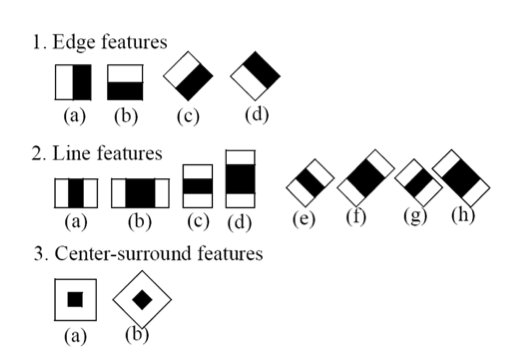
\includegraphics[width=0.6\textwidth]{media/classification/viola-jones-features.png}
    \caption{Examples of Haar-like features used in the Viola-Jones framework.}
\end{figure}

\paragraph{Integral Image Representation}
An integral image enables $O(1)$ computation of pixel sums in any rectangular region. It stores the cumulative sum of pixel intensities above and to the left of a point $(x,y)$:
\begin{equation}
    II(x, y) = \sum_{x' \leq x, y' \leq y} I(x', y')
\end{equation}

\begin{figure}[H]
    \centering
    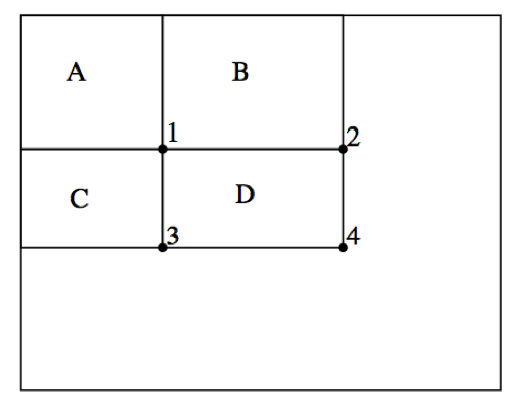
\includegraphics[width=0.6\textwidth]{media/classification/integral-image.png}
    \caption{Integral image representation for fast computation of Haar-like features.}
\end{figure}

Using the integral image, the sum of region $D$ (bottom-right) requires only four array references:
\[
    \text{Sum}(D) = \underbrace{II(x_4, y_4)}_{\text{A + B + C + D}} - \underbrace{II(x_2, y_2)}_{\text{A + B}} - \underbrace{II(x_3, y_3)}_{\text{A + C}} + \underbrace{II(x_1, y_1)}_{\text{A}}
\]
Because it relies on cumulative sums, the integral image is computed highly efficiently in a single pass over the original image.

\paragraph{Classifiers - AdaBoost}
Viola-Jones typically relies on \textbf{AdaBoost}, an ensemble method that builds a strong classifier by combining multiple weak classifiers ($h_t(x)$):
\[ f(x) = \sum_{t=1}^{T} \alpha_t h_t(x) \]
where $\alpha_t$ is the weight based on training performance. The final output is $\text{sign}(f(x))$. AdaBoost trains iteratively, selecting optimal weak classifiers while increasing the weights of misclassified samples to focus the model on difficult cases.

\paragraph{Classifier Cascade}
To optimize detection speed, Viola-Jones uses a sequence (cascade) of binary classifiers. Each stage analyzes an image window; if a classifier predicts "non-object," the window is immediately discarded. This early rejection of negative samples drastically reduces overall computational cost.